\chapter{Results}


\section{Irradiation}

After explaining the theoretical background of the problem and introducing the approach behind the simulations, we can now present the results obtained for the model we have developed. The results will always come in pairs, as we have done the same simulations for both the original model, where the frequency factor stays in a constant value (which we will call temperature independent), and the one we propose, where the frequency factor is a function of the temperature following equation \ref{eq:freqfactor_lnT} (temperature dependent). For this first section, we will focus on the graphs obtained from the simulations of the \textit{irradiation} stage of the material. These can be seen in Figures \ref{fig:irradiation_nievolution}-- \ref{fig:irradiation_chneutrality}

\begin{figure}
    \centering
    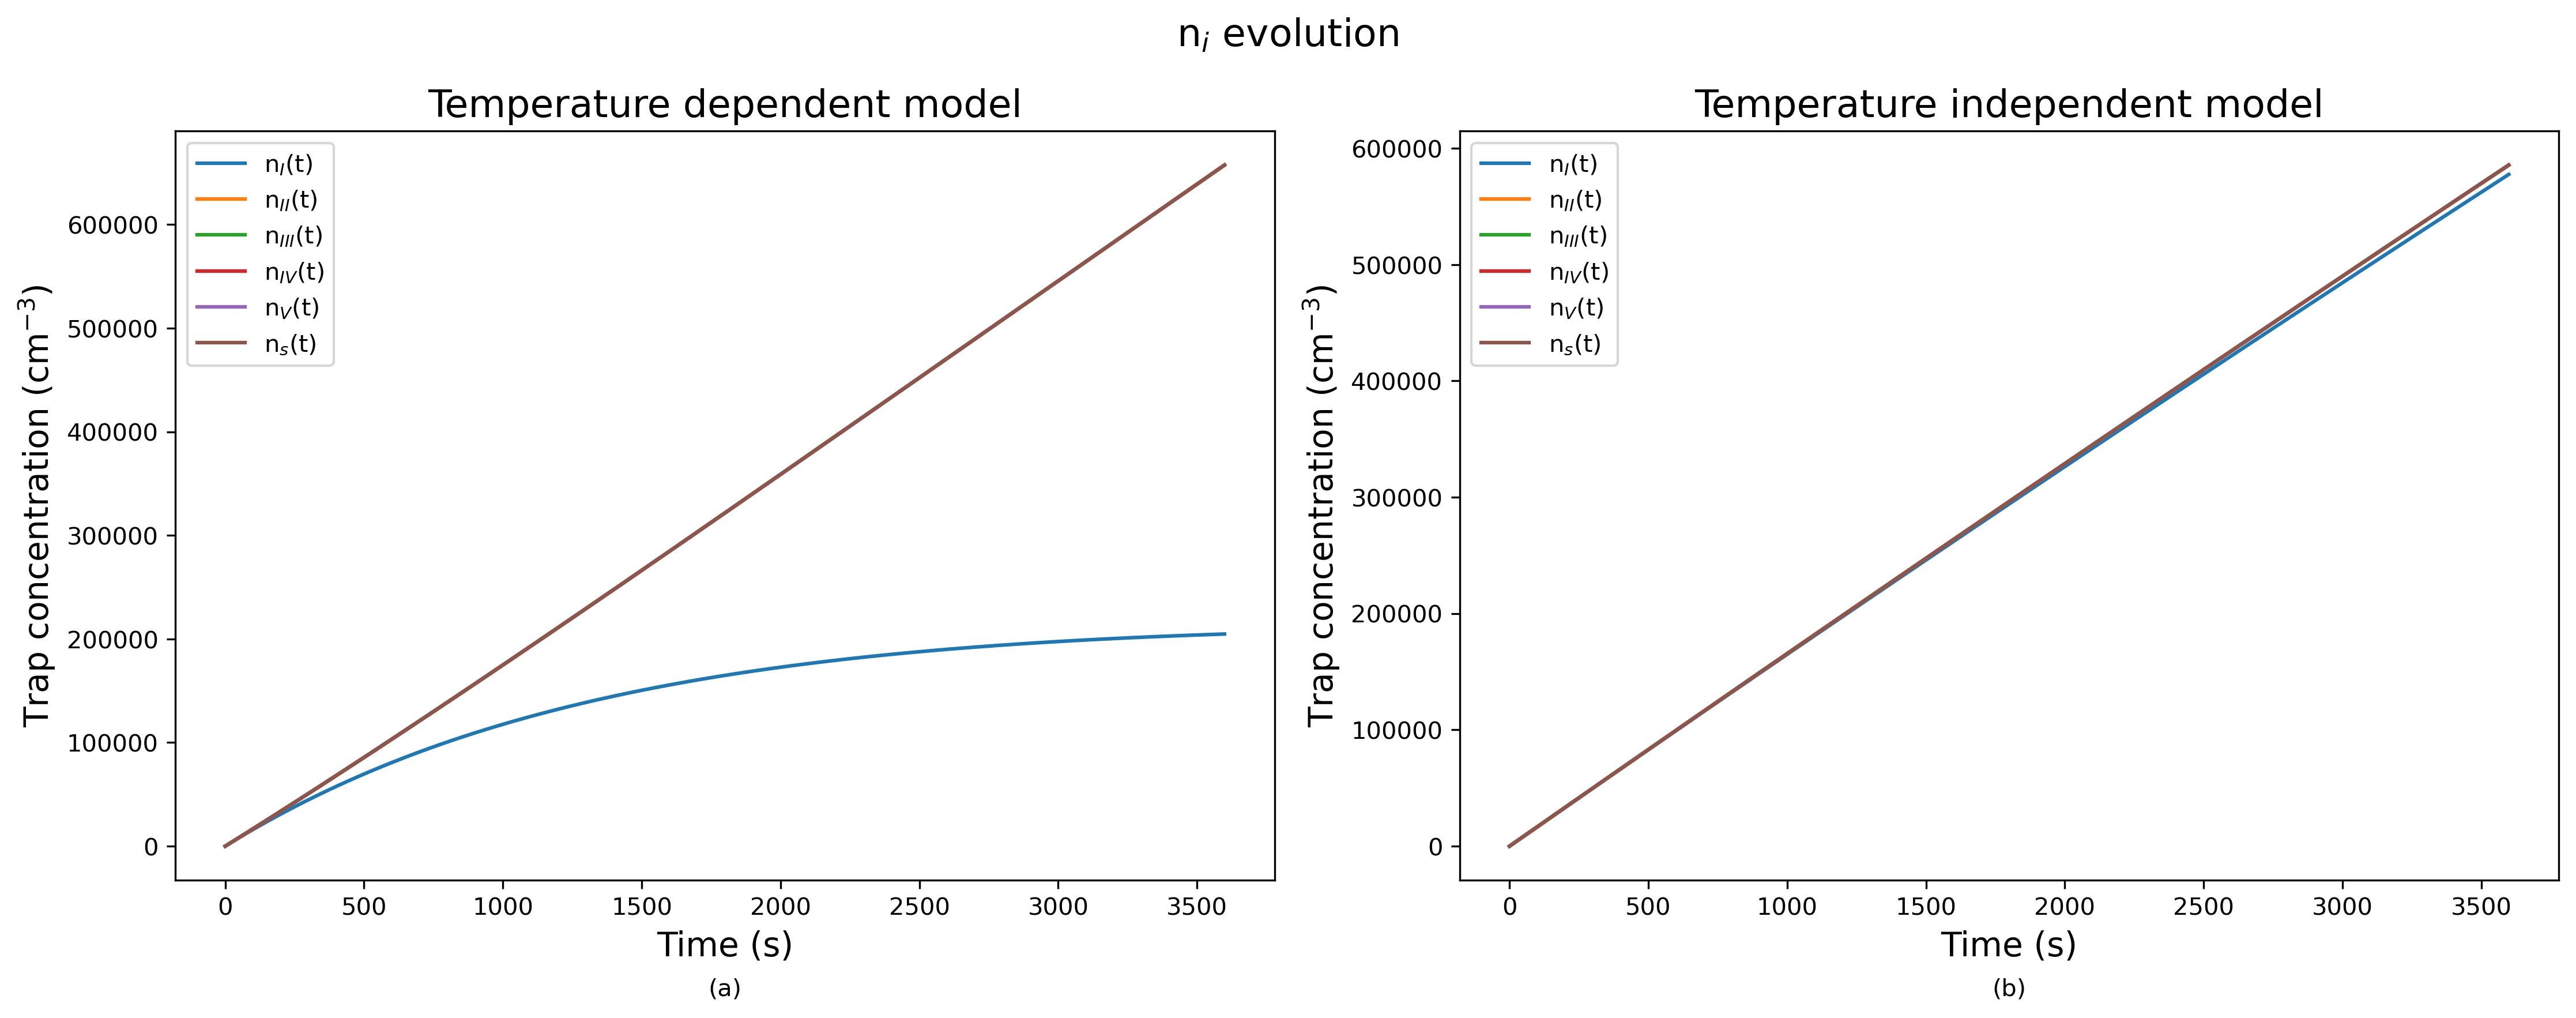
\includegraphics[width=\textwidth]{Images/Irradiation n_i evolution.png}
    \caption{Evolution of trap concentrations $n_i(t)$  plotted against time for the LiF:Mg, Ti during the irradiation phase for both models (a) Temperature dependent model, where the probabilities of excitation vary with temperature; (b) Temperature independent model, where the excitation probabilities are fixed parameters. Both were subjected to a constant irradiation rate of $G = 1000$ cm$^{-3}$ s$^{-1}$ and a laboratory temperature of $T = 25$ \textdegree C during 3600 seconds. The traps are labeled as follows: I (blue), II (orange), III (green), IV (red), V (purple), and s (brown).}
    \label{fig:irradiation_nievolution}
\end{figure}

\vspace{10pt}

First and foremost, we can start our analysis of the irradiation stage by looking at the evolution of the occupancy of the traps $n_i$ as a function of time. In Figure \ref{fig:irradiation_nievolution} it is shown that the most prominent difference between the two models lies in what occurs with the trap I, shown by the blue line of $n_I$. In the temperature independent model, we see that all traps behave in a very similar way; they get gradually filled over time, as the electron-hole pairs are generated. There is a perceptible downward curve in the end of the irradiation time for the $n_I$ trap, which could hint that the trap is being filled to its maximum capacity, but it is not very clear. In the temperature dependent model however, we see that the filling of the $n_I$ trap is much more noticeable, and in turn the growth of the rest of the traps is more pronounced. We see that, without a doubt, the trap I is saturated in the first few minutes of irradiation. % y qué pasa con la inclinación de la curva??

\begin{figure}
    \centering
    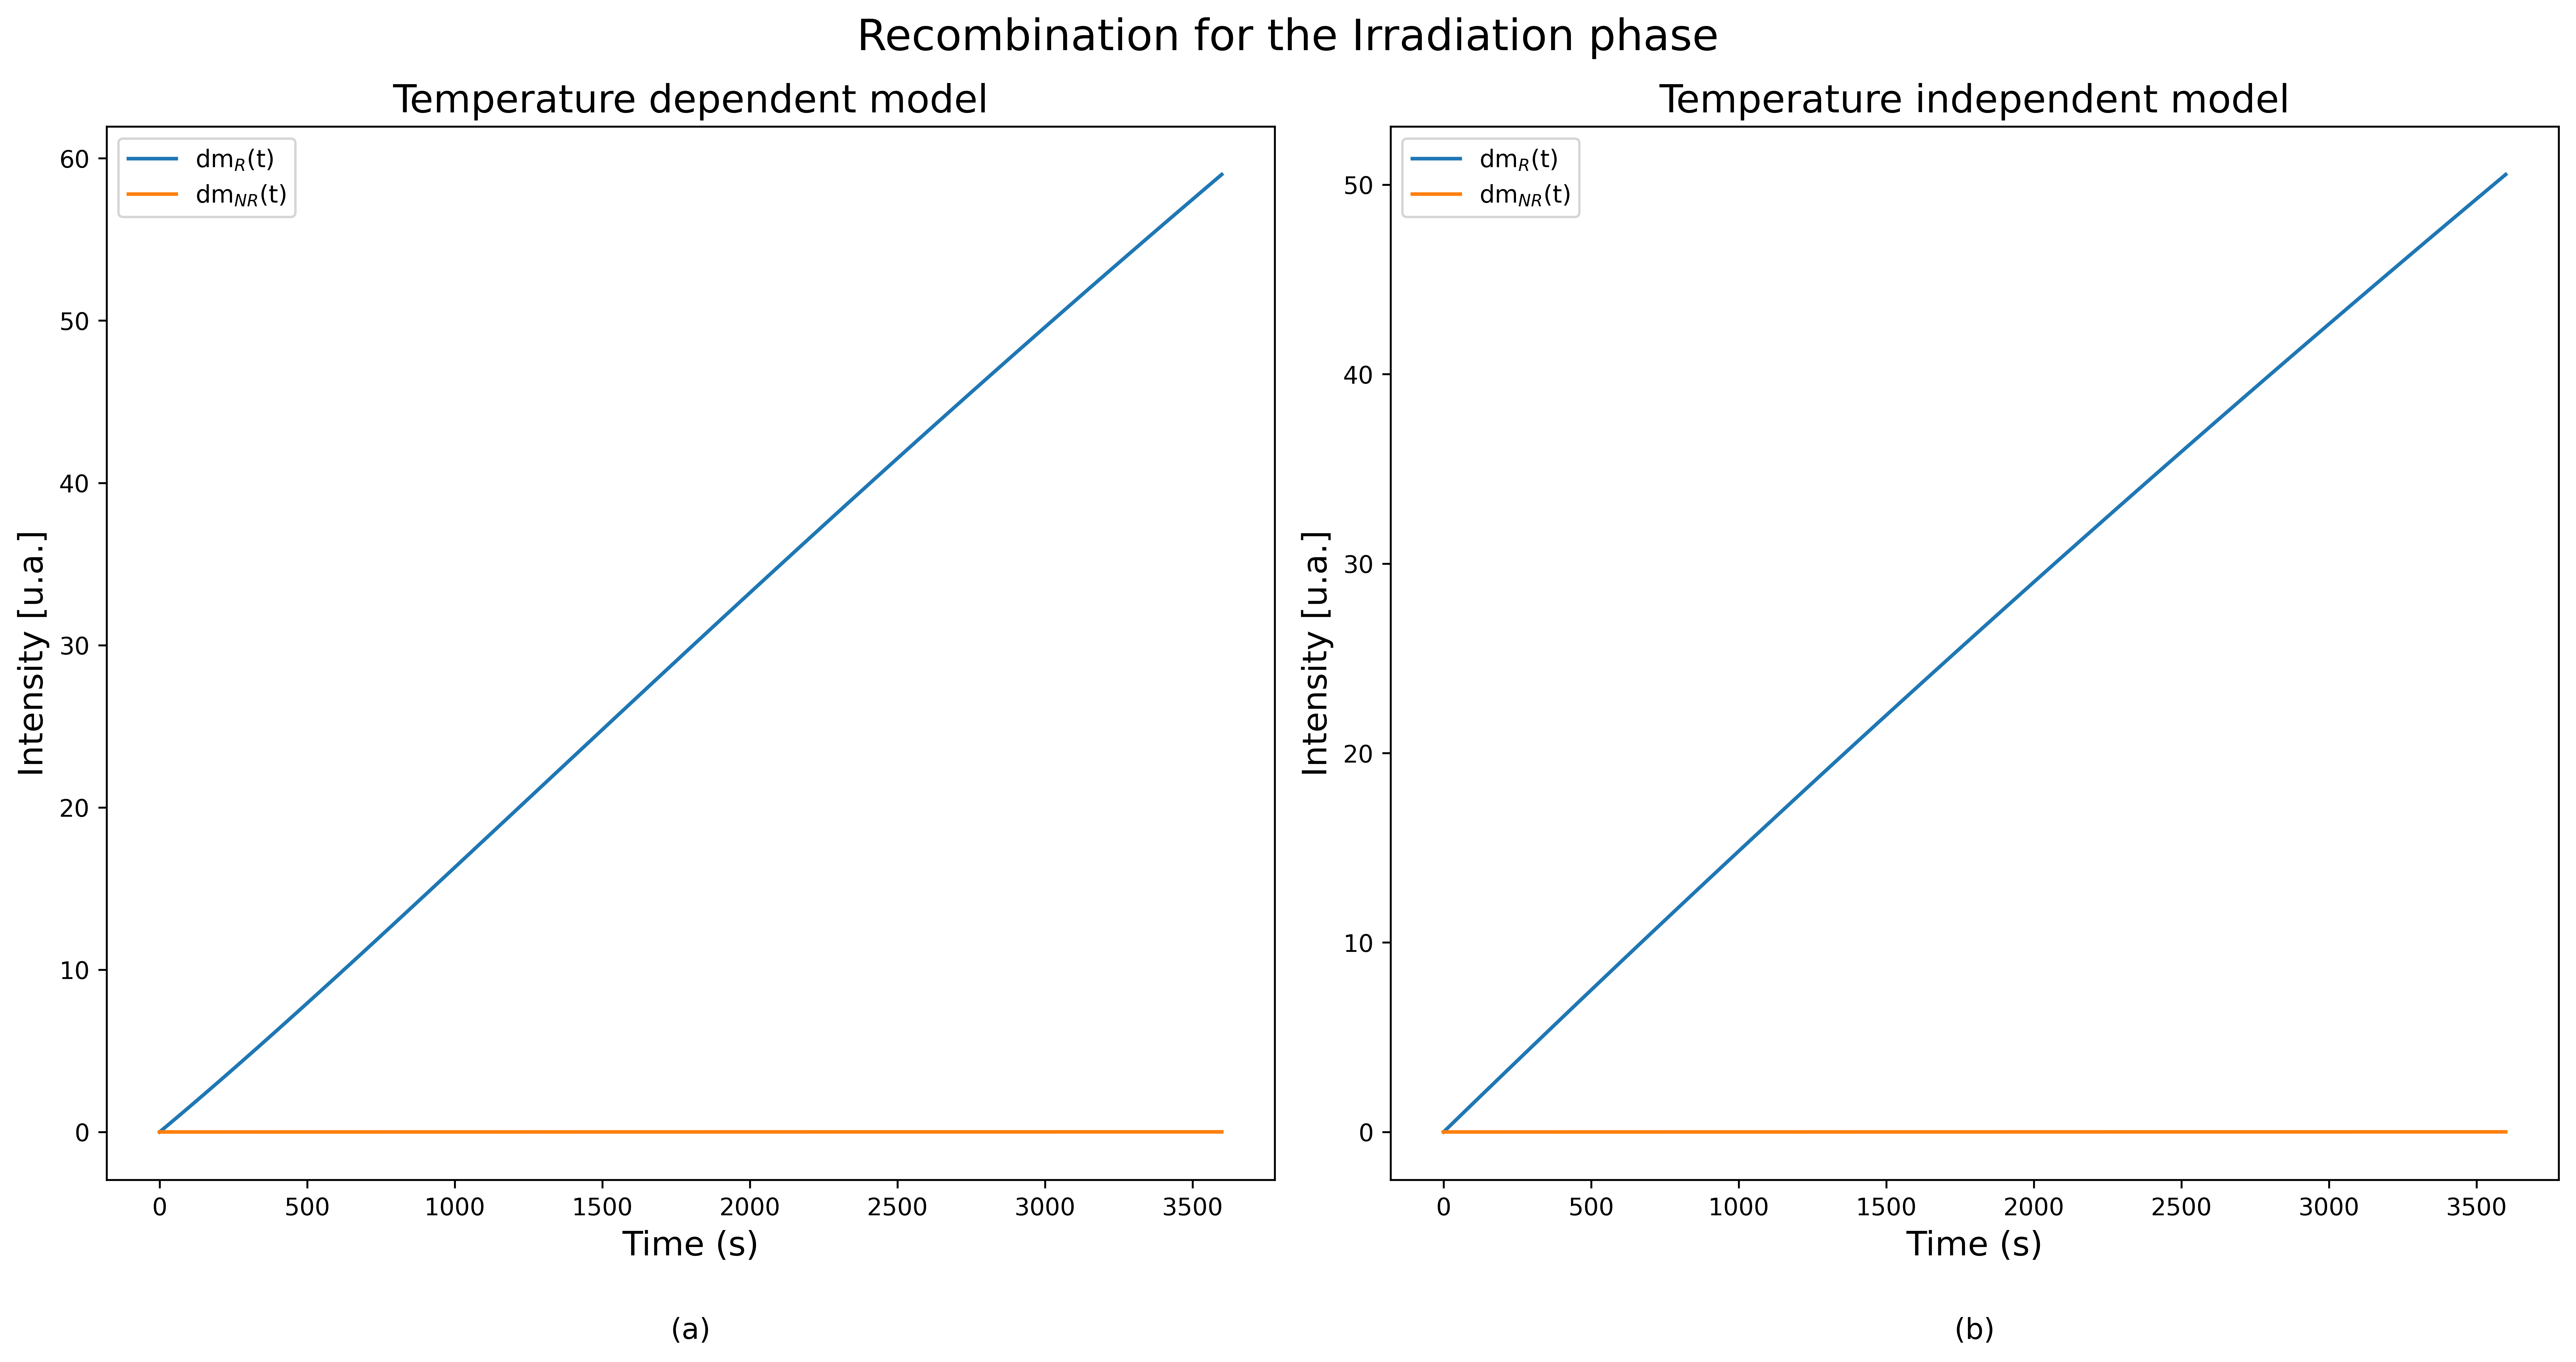
\includegraphics[width=\textwidth]{Images/Irradiation Recombination.png}
    \caption{Recombination rates during the irradiation phase for both models. (a) Temperature-dependent model; (b) Temperature-independent model. The plotted quantities correspond to the radiative ($dm_R/dt$) and non-radiative ($dm_{NR}/dt$) recombination rates. Both models were subjected to a constant irradiation rate of $G = 1000$ cm$^{-3}$ s$^{-1}$ and a laboratory temperature of $T = 25$ \textdegree C during 3600 seconds.}
    \label{fig:irradiation_recombination}
\end{figure}

\vspace{10pt}

If we look at recombination rates, in Figure \ref{fig:irradiation_recombination} we can see that both models show a very similar behavior, with the exception of the steep of growth of the radiative recombination rate. In the temperature independent model, the growth is slowed compared to the temperature dependent model, indicating a higher trap occupation. Overall, it is a similar behavior than the one seen in \ref{fig:irradiation_nievolution}, as it can be explained with the same principle. When making the frequency factor dependent of temperature, thermal energy dynamics are added, which facilitates the excitation and mobility of our charged carriers. This leads to a higher occupation of traps ---beginning with the one closer to the Fermi level, trap I---, which mathematically translates to higher slope in the graphs. 
Also, the nearly flat and negligible $dm_{NR}(t)$ in both cases suggests that non-radiative processes play a minimal role under these conditions. % ??? why???

\vspace{10pt}

The last graph to analyze is the one introduced in Section \ref{sec:simulations} to validate the model. In Figure \ref{fig:irradiation_chneutrality} we can see that both models satisfy the charge neutrality condition, as the total positive and negative charges are approximately equal at all times. The small deviation from the ideal value of 1 is on the order of $10^{-6}$, which is negligible and can be attributed to numerical errors in the simulations. This confirms that the model is consistent with the physical principles of charge conservation as introduced in equation \ref{eq:charge_neutrality}, and that the simulations have been done correctly.

\begin{figure}
    \centering
    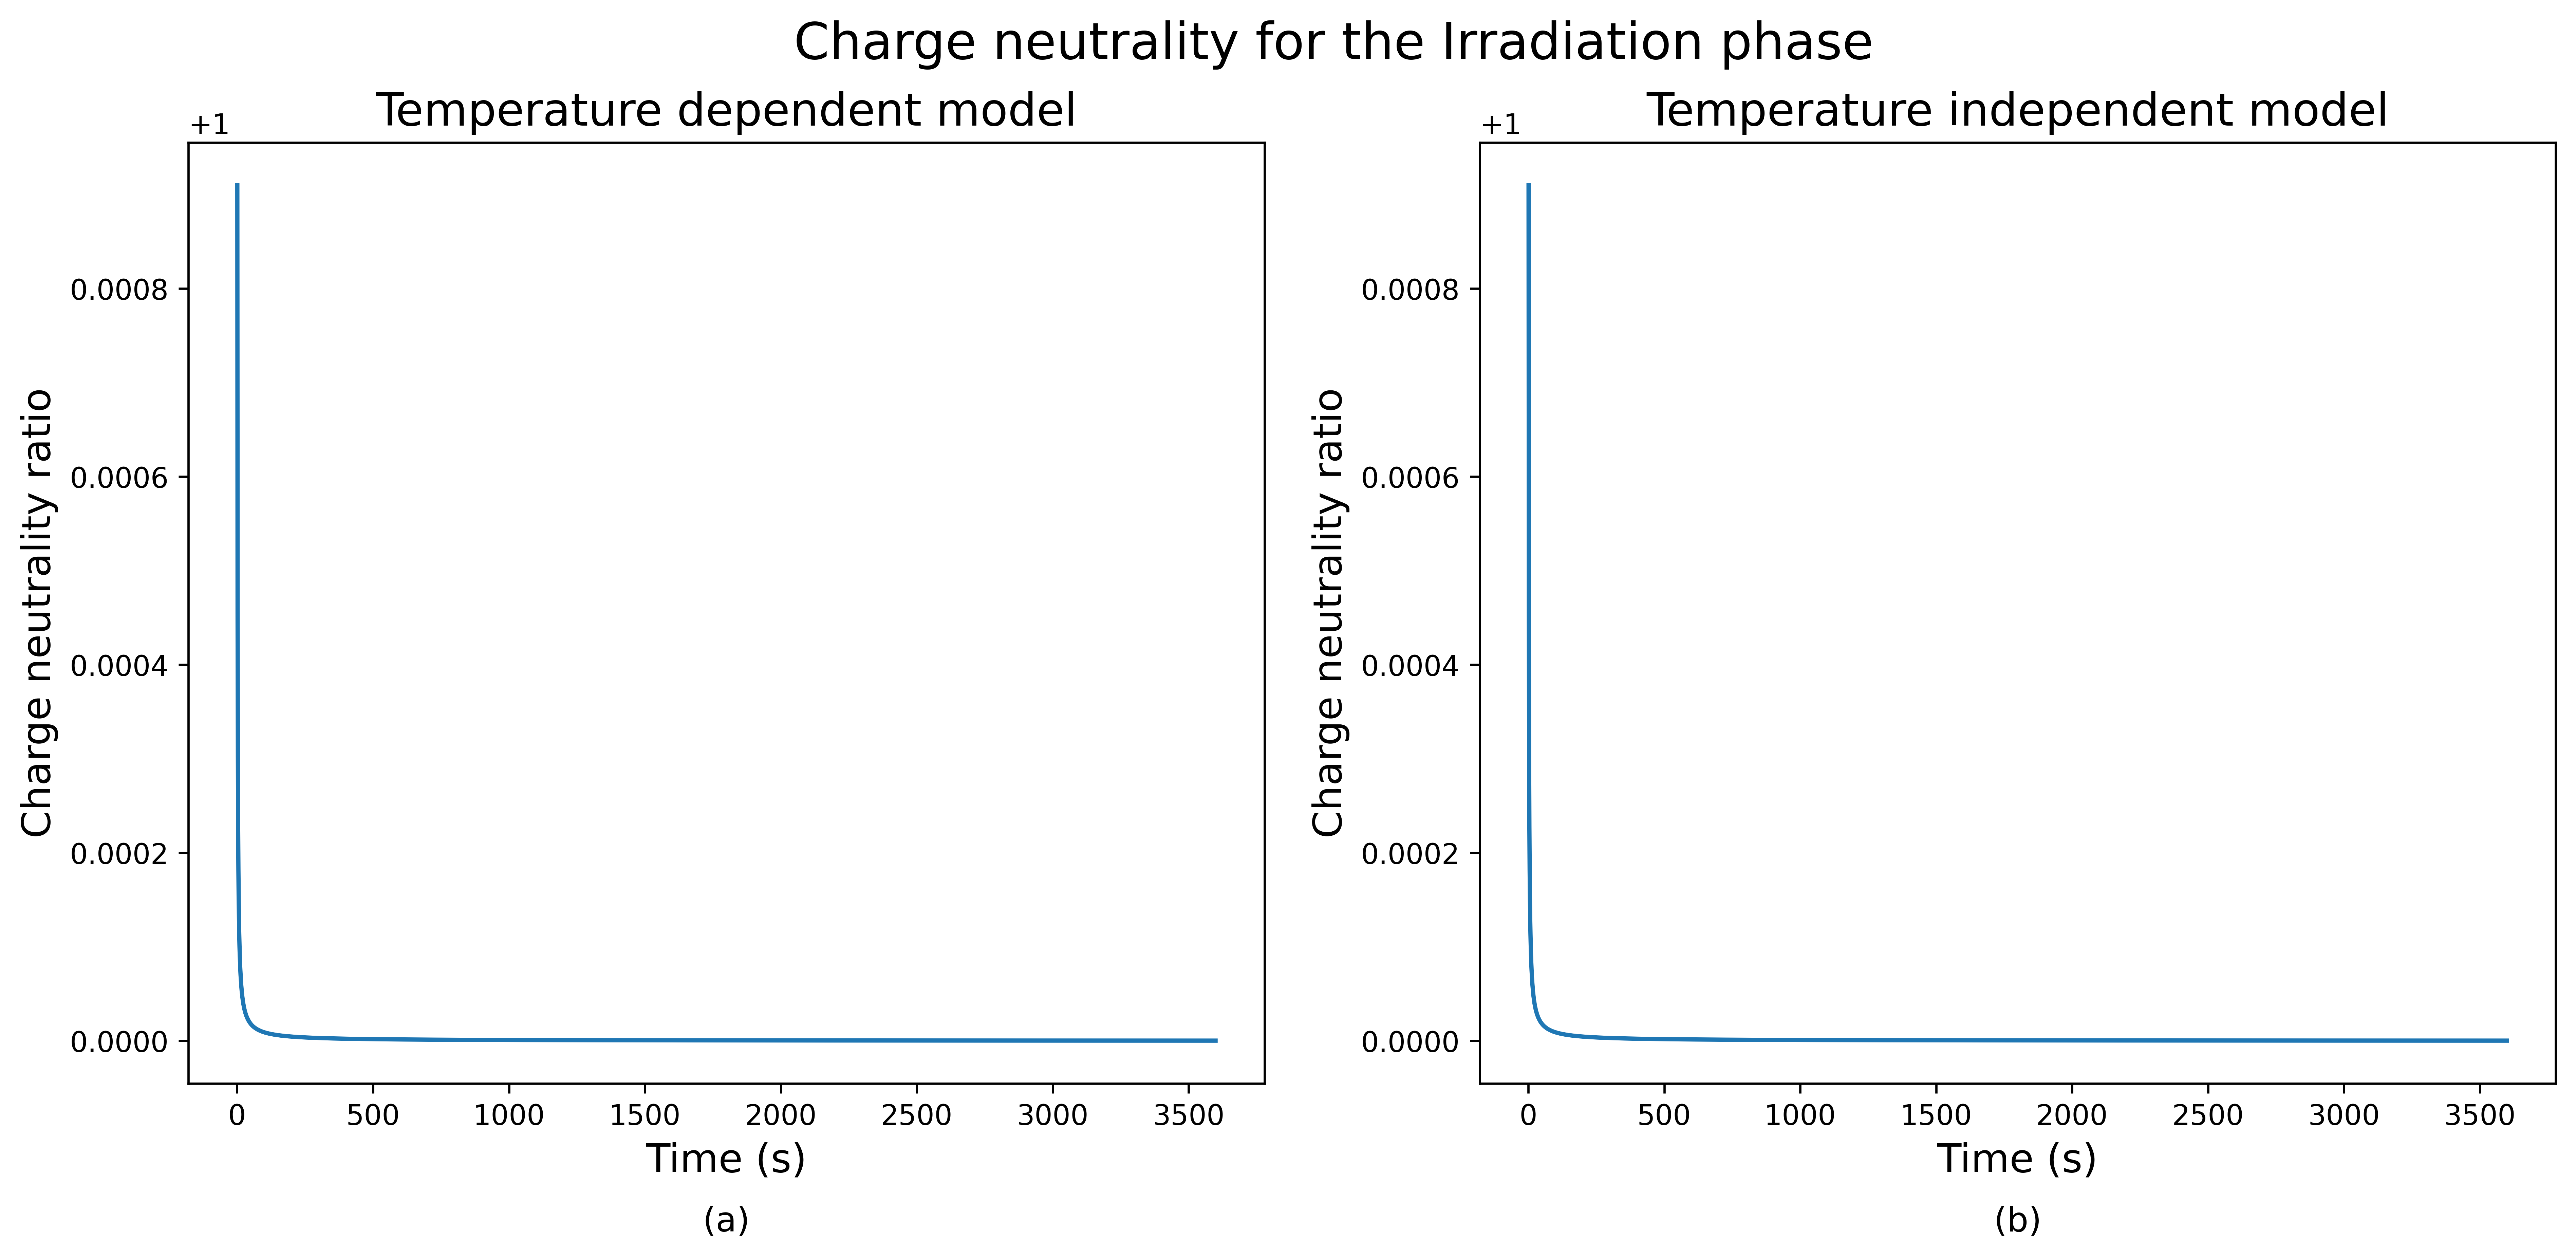
\includegraphics[width=\textwidth]{Images/Irradiation Charge neutrality.png}
    \caption{Charge neutrality ratio for the LiF:Mg, Ti plotted against temperature during the irradiation phase for both models. (a) Temperature dependent model; (b) Temperature independent model. The plotted ratio corresponds to the total negative charge divided by the total positive charges in the system. Both simulations were performed under a constant generation rate of $G = 1000$ cm$^{-3}$ s$^{-1}$ and a laboratory temperature of $T = 25$ \textdegree C during 3600 seconds.}
    \label{fig:irradiation_chneutrality}
\end{figure}

\section{Relaxation}

After the irradiation stage, we can now analyze the results obtained from the \textit{relaxation} stage of the material. The graphs obtained from the simulations can be seen in Figures \ref{fig:relaxation_nievolution}--\ref{fig:relaxation_chneutrality}.

\vspace{10pt}

Again, the graphs will be presented in pairs, one for the temperature independent model and one for the temperature dependent model. The first graph to analyze is the evolution of the occupancy of the traps $n_i$ as a function of time, which can be seen in Figure \ref{fig:relaxation_nievolution}. At a first glance, one can clearly see a difference between the two figures, divided by one main factor: how does the detrapping work. By keeping the laboratory temperature at a fixed value, the probability of thermal detrapping is constant over time, and without electron-hole pair generation, the system evolves solely through the release of previously trapped carriers. % por qué entonces la trampa I se vacía y las otras no?
As a result, the relaxation dynamics are governed by the intrisic properties of each trap ---specifically the activation energy and frequency factor---, which determine how trapped carriers will evolve. 

\vspace{10pt}

\begin{figure}
    \centering
    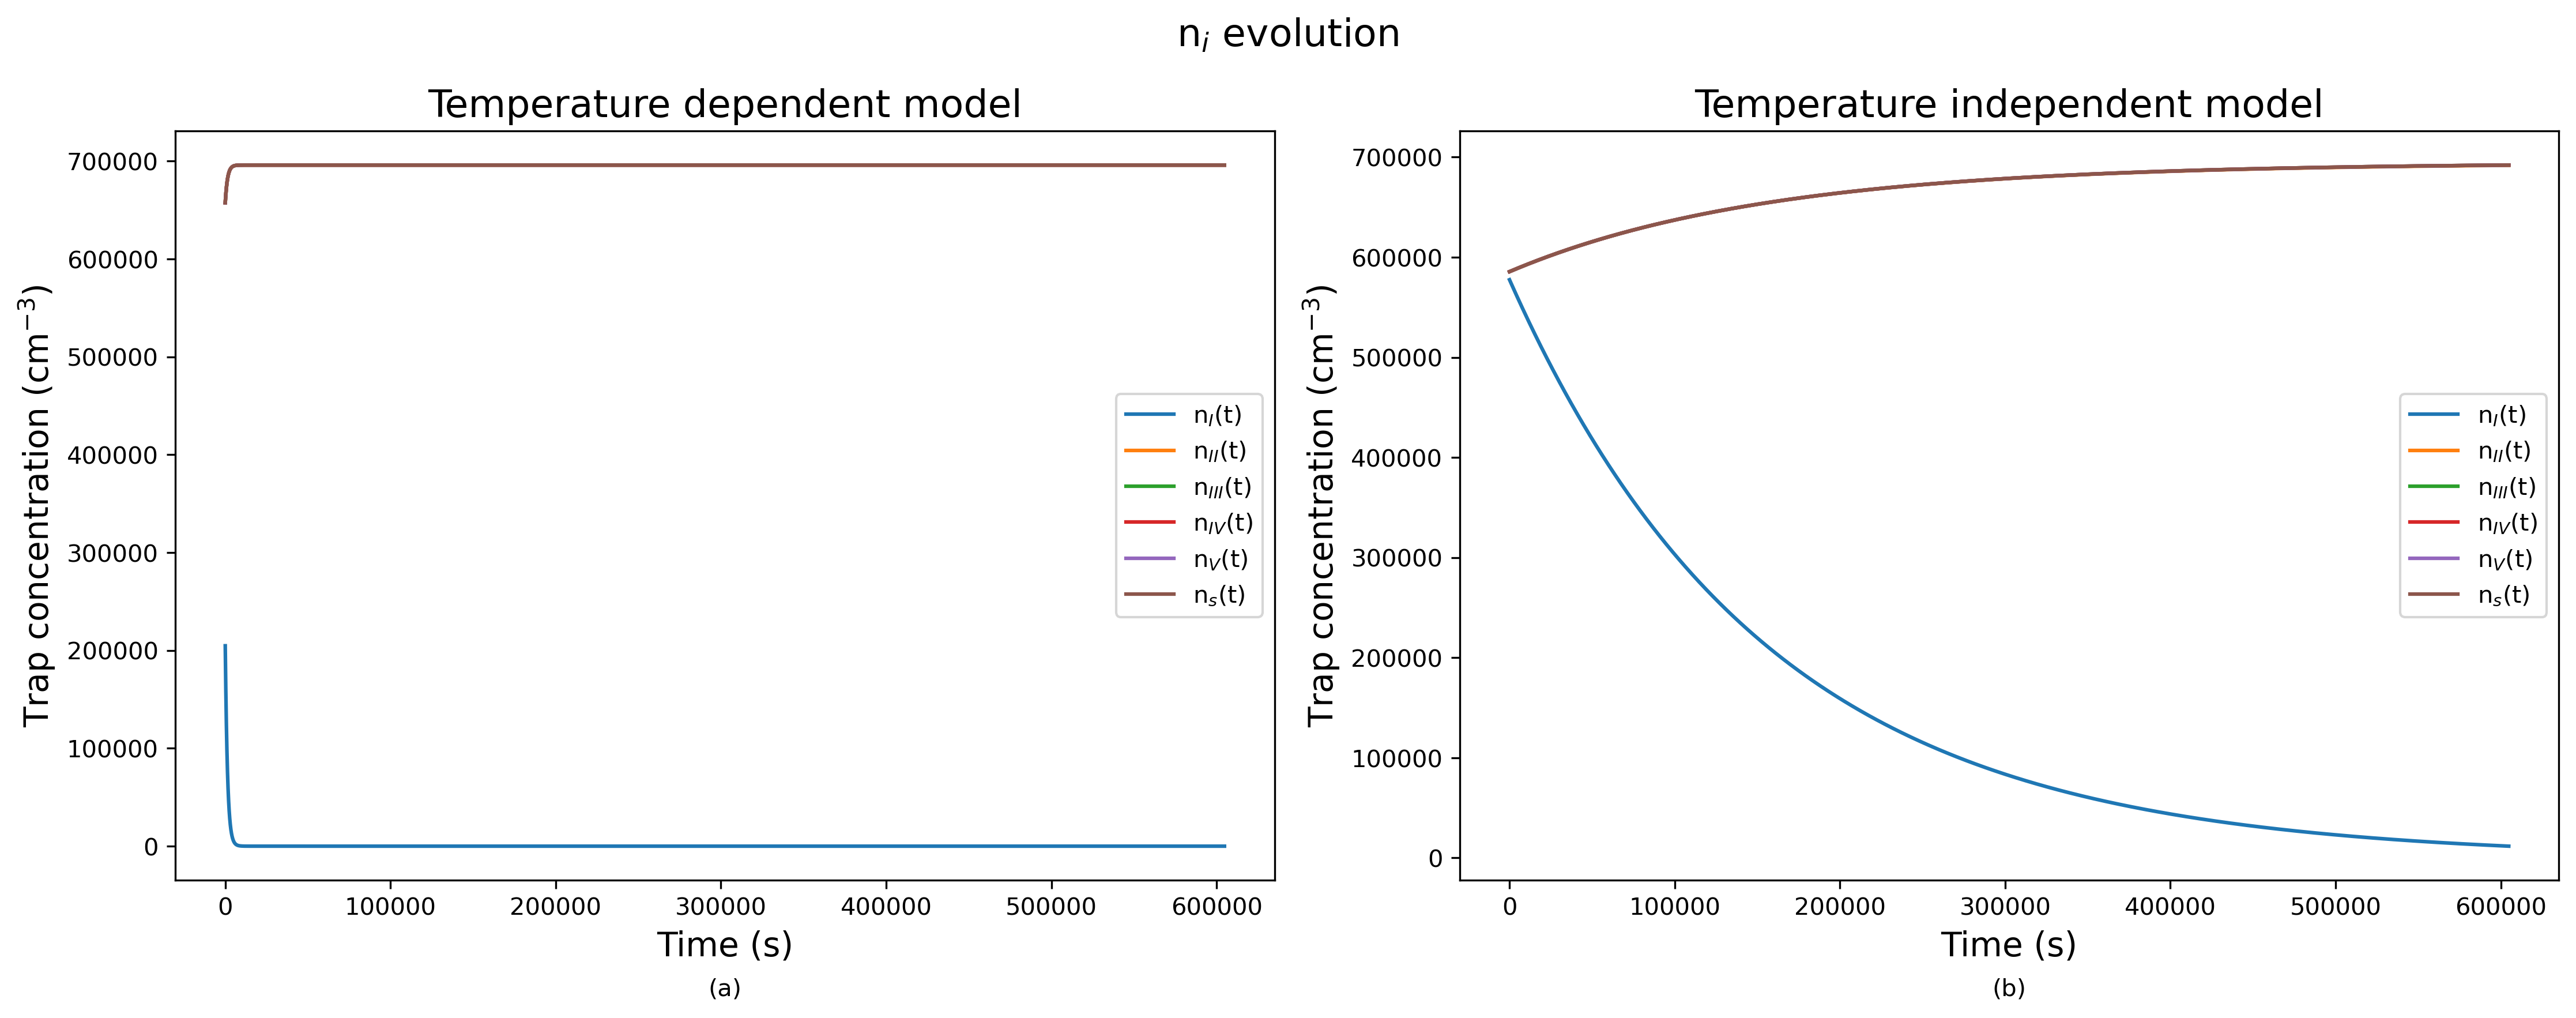
\includegraphics[width=\textwidth]{Images/Relaxation n_i evolution.png}
    \caption{Evolution of trap concentrations $n_i(t)$  plotted against time for the LiF:Mg, Ti during the relaxation phase for both models (a) Temperature dependent model; (b) Temperature independent model. Both were subjected to a constant generation rate of $G = 0$ cm$^{-3}$ s$^{-1}$ and a laboratory temperature of $T = 25$ \textdegree C during 604,800 seconds. The traps are labeled as follows: I (blue), II (orange), III (green), IV (red), V (purple), and s (brown).}
    \label{fig:relaxation_nievolution}
\end{figure}

The decay of the trap I in both models is attributed to the fact that it is the closest trap to the Fermi level, and therefore the one with the lowest activation energy. This means that, even though the frequency factor is constant in the temperature independent model, the carriers will still be able to escape from this trap more easily than from the others. In the temperature dependent model we see that the decay of trap I is much more pronounced, as the thermal dynamics allow for a higher probability of detrapping. The other traps, on the other hand, remain mostly unaffected due to their deeper energy levels, which result in significantly lower detrapping probabilities at the laboratory temperature. This contrast highlights the selective sensitivity of shallow traps to a certain thermal activation temperature, while deeper traps retain their occupancy over longer timescales. It also explains the need for a third stage of the process, where this temperature would be increased to allow the detrapping of all the excited electrons and holes and returning to the equilibrium state from the metastable state the material finds itself in after the relaxation phase.

\begin{figure}
    \centering
    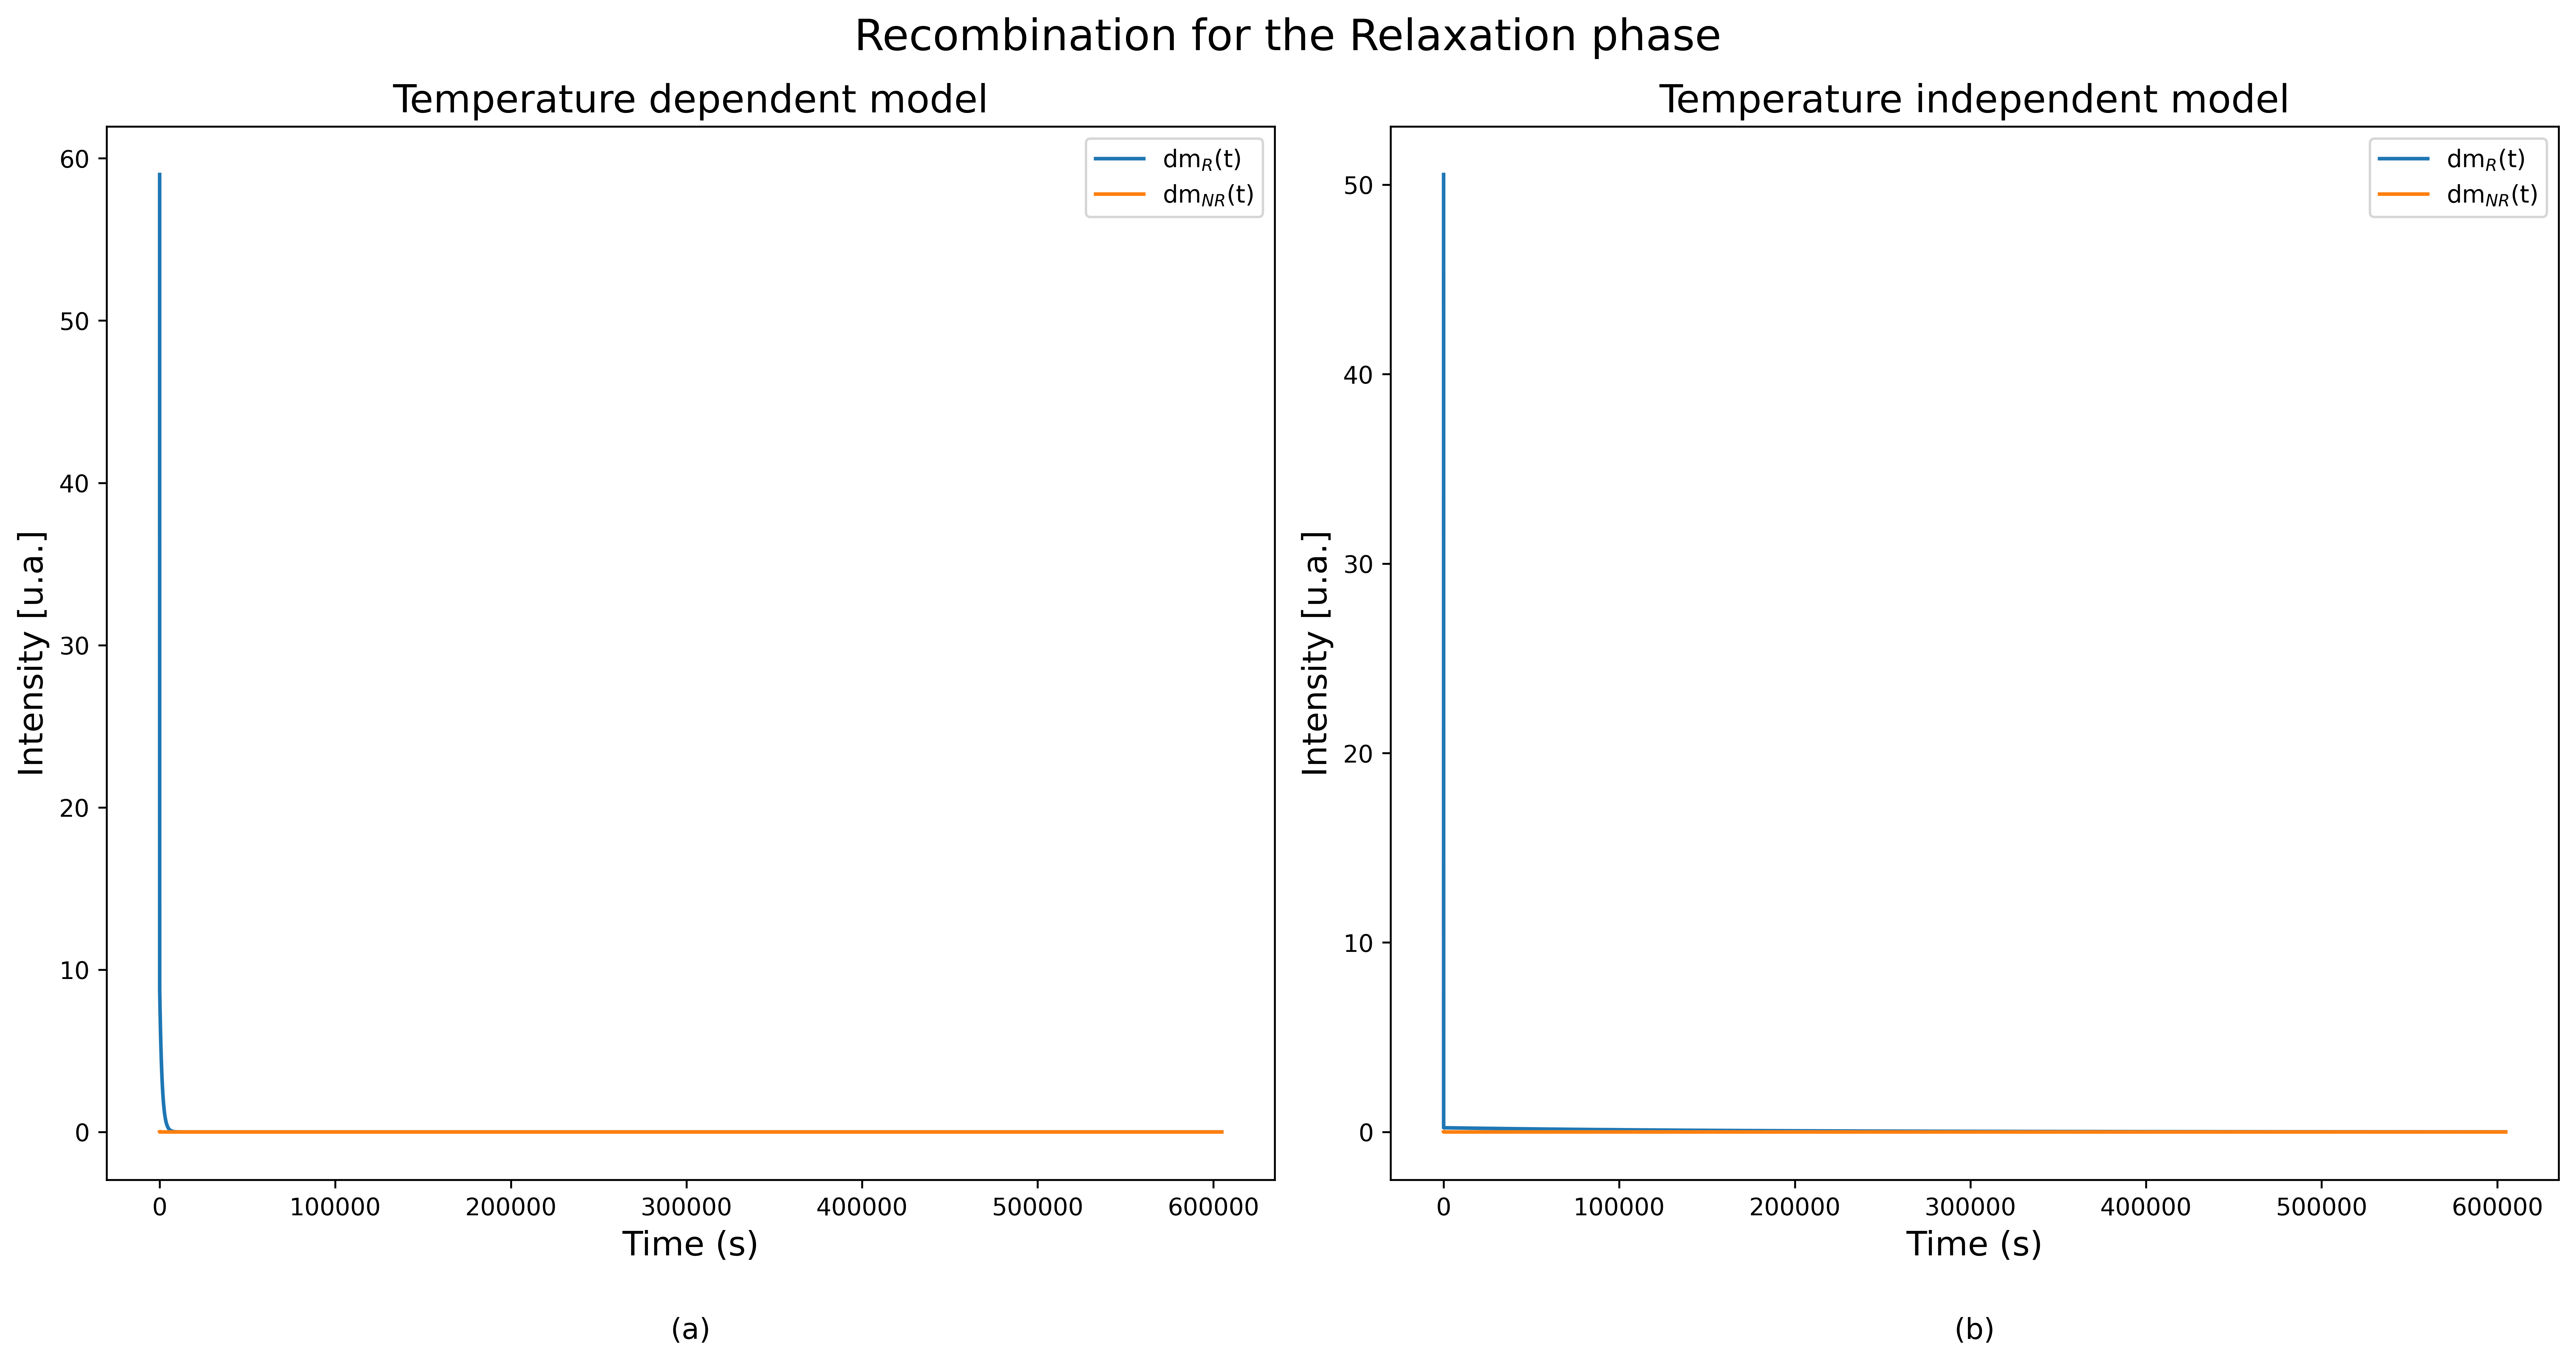
\includegraphics[width=\textwidth]{Images/Relaxation Recombination.png}
    \caption{Recombination rates for the LiF:Mg, Ti during the relaxation phase for both models. (a) Temperature dependent model; (b) Temperature independent model. The plotted quantities correspond to the radiative ($dm_R/dt$) and non-radiative ($dm_{NR}/dt$) recombination rates. Both models were subjected to a constant generation rate of $G = 0$ cm$^{-3}$ s$^{-1}$ and a laboratory temperature of $T = 25$ \textdegree C during 604,800 seconds.}
    \label{fig:relaxation_recombination}
\end{figure}

\vspace{10pt}

The next graph to analyze is the one showing the recombination rates during the relaxation stage, which can be seen in Figure \ref{fig:relaxation_recombination}. In this stage, the recombination rate $dm_{R(t)}$ exhibits a sharp decay in both models, consistent with the rapid depletion of free carriers following the irradiation stop. This behavior is driven by the thermal detrapping from the shallow traps --like the trap I we mentioned in the previous paragraph---, which quickly empties when stabilizing the laboratory temperature. Again, the nearly flat $dm_{NR}(t)$ in both cases suggests that non-radiative processes play a minimal role under these conditions.

\vspace{10pt}

Although the overal shape of the curves is similar, the temperature dependent model shows a more pronounced decay in the radiative recombination rate. This is due to the fact that, as we have seen in the previous section, the temperature dependent model allows for a higher occupation of traps, which leads to a higher probability of recombination. This is consistent with the fact that the temperature dependent model has a higher slope in the $n_i$ evolution graph, as we saw in Figure \ref{fig:irradiation_nievolution}.

\vspace{10pt}

The charge neutrality plots shown in Figure \ref{fig:relaxation_chneutrality} confirm that the model preserves global charge conservation throughout the relaxation phase. Both the temperature independent and dependent model maintain a nearly perfect balance between positive and negative charges, with only a negligible deviation on the order of $10^{-6}$ at early times. The stability of these two plots supports the robustness of the simulations done for this phase, and reinforces the consistency of the relaxation dynamics.

\begin{figure}
    \centering
    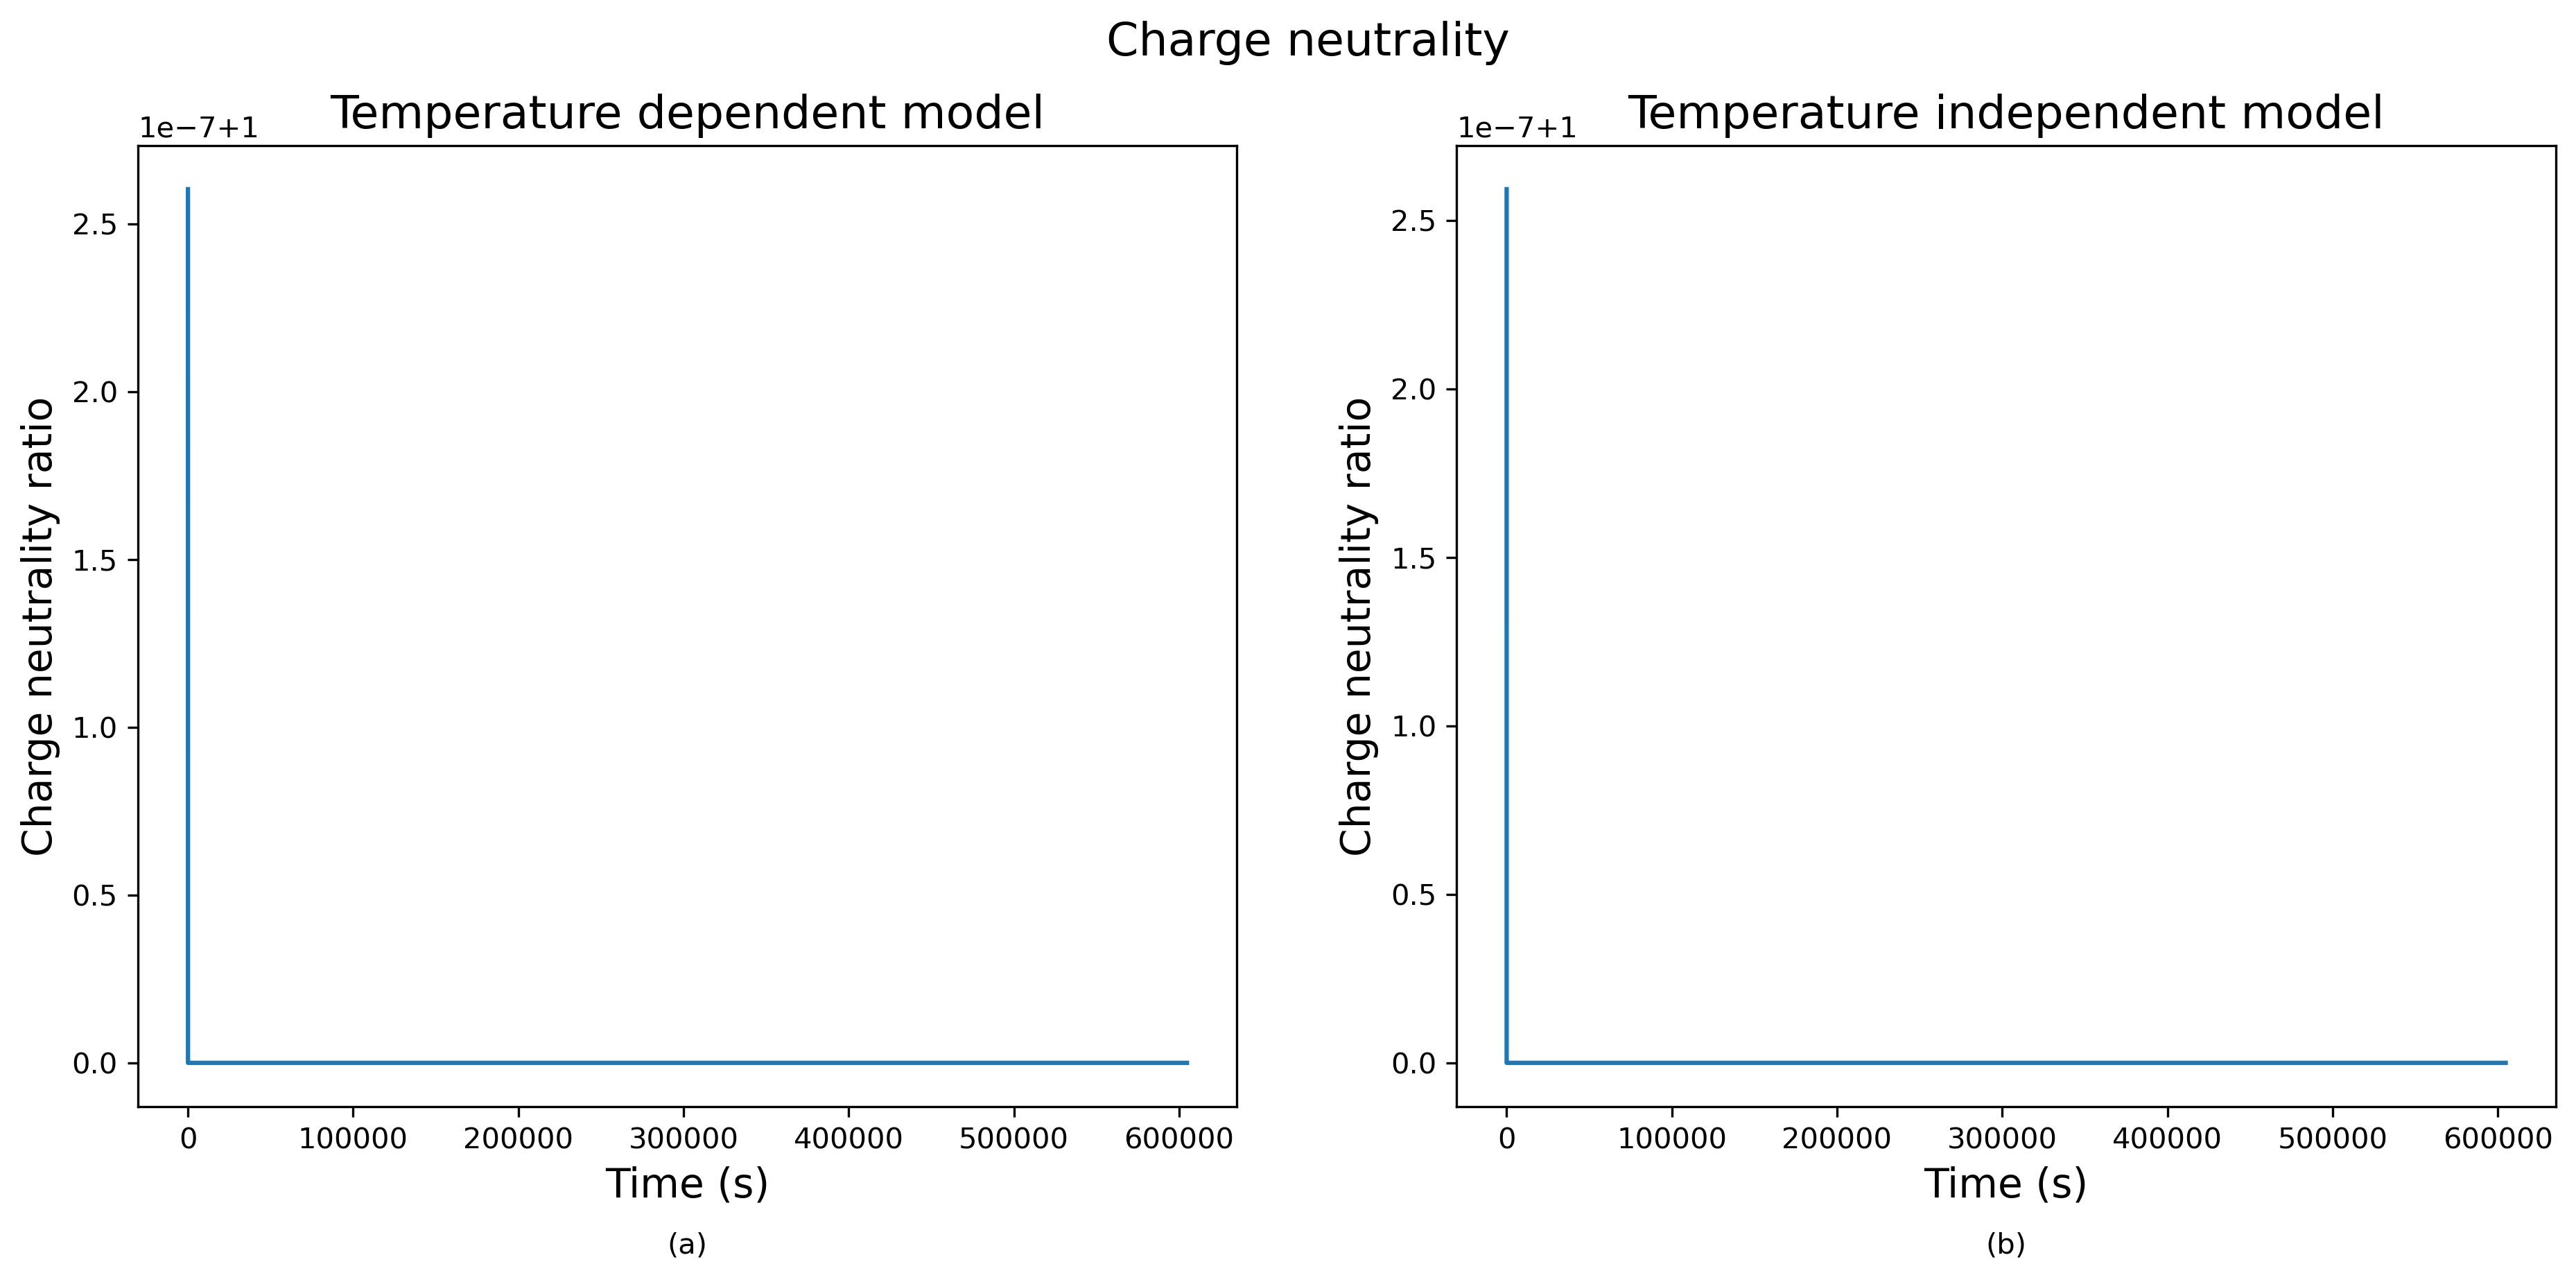
\includegraphics[width=\textwidth]{Images/Relaxation Charge neutrality.png}
    \caption{Charge neutrality ratio for the LiF:Mg, Ti plotted against temperature during the relaxation phase for both models. (a) Temperature dependent model; (b) Temperature independent model. The plotted ratio corresponds to the total negative charge divided by the total positive charges in the system. Both simulations were performed under a constant generation rate of $G = 0$ cm$^{-3}$ s$^{-1}$ and a laboratory temperature of $T = 25$ \textdegree C during 604,800 seconds.}
    \label{fig:relaxation_chneutrality}
\end{figure}

\vspace{10pt}

\section{Heating}\label{sec:heating}

We can now move onto the last stage of the process, the \textit{heating} stage. Here we will obtain the previously introduced TL glow curve, as one of the graphs we have been doing so far. The results obtained from the simulations in this section can be seen in Figures \ref{fig:GC_ActivationAndPeakTemperatures}--\ref{fig:heating_chneutrality}. 

\begin{figure}[ht]
    \centering
    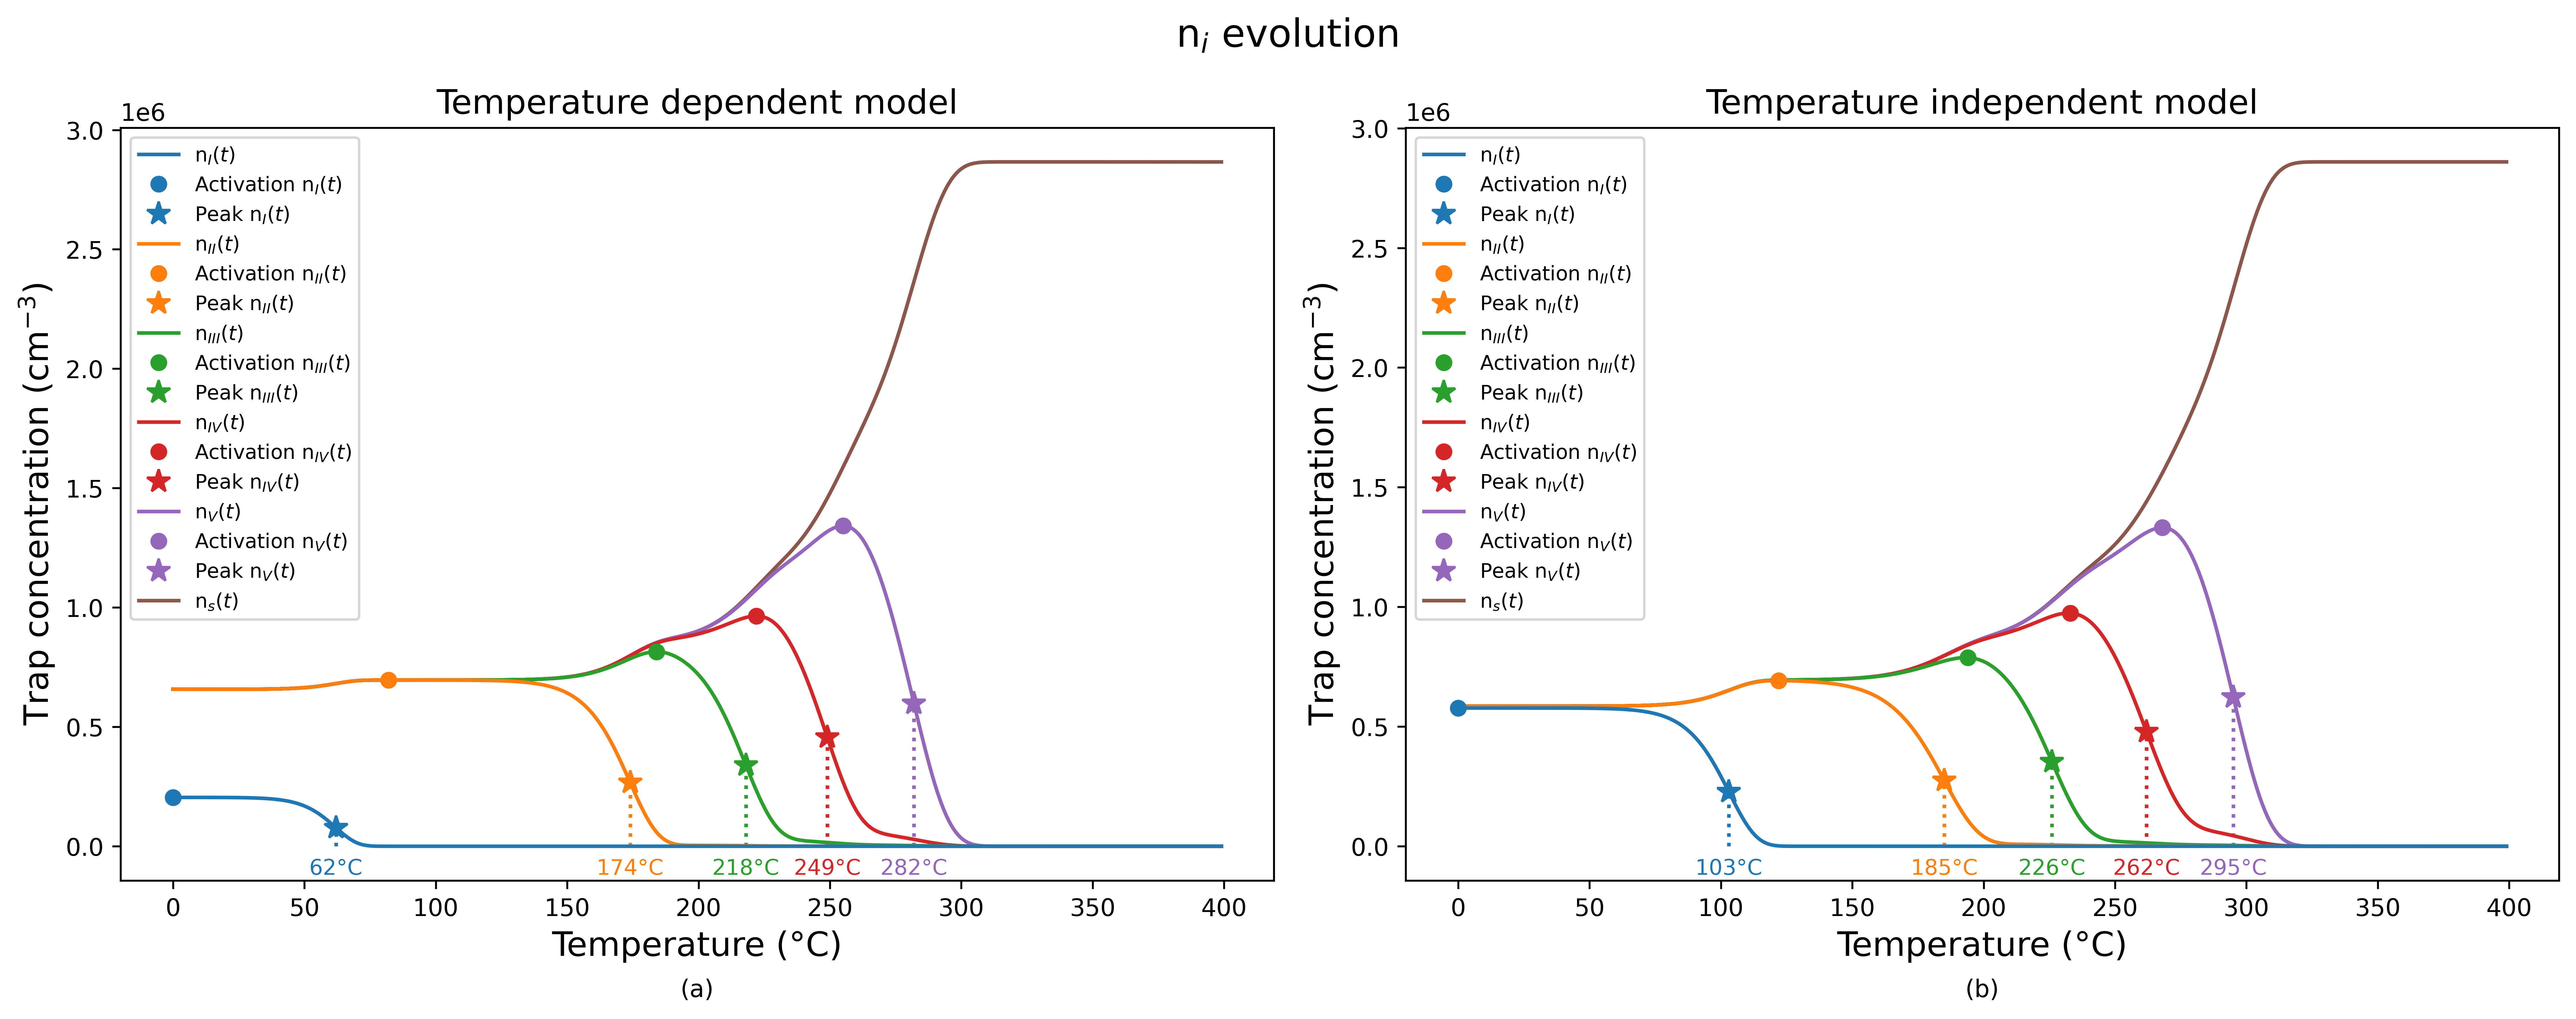
\includegraphics[width=\textwidth]{Images/GC_ActivationAndPeakTemperatures.png}
    \caption{Evolution of trap concentrations $n_i(t)$ for the LiF:Mg, Ti plotted against temperature during the heating phase for both models. (a) Temperature dependent model; (b) Temperature independent model. For each trap, both the activation temperature (filled circle) and peak temperature (star icon) are indicated. The peak temperature has a dotted line that reaches the X axis and indicates the specific value for each trap. The simulations were performed under a constant generation rate of $G = 0$ cm$^{-3}$ s$^{-1}$ and an increasing laboratory temperature from 0 \textdegree C to 400 \textdegree C during 400 seconds. The traps are labeled as follows: I (blue), II (orange), III (green), IV (red), V (purple), and s (brown).}
    \label{fig:GC_ActivationAndPeakTemperatures}
\end{figure}

\vspace{10pt}
Before the TL glow curve, we must first analyze what is happening with the occupancy of the traps. Taking now the temperature in our X axis, we can see at a first glance in Figure \ref{fig:GC_ActivationAndPeakTemperatures}, that both models show a similar behavior. As expected, the trap I is the first one to be emptied as it is the closest to the Fermi level. And as it has been seen, it is also here where we see the most significant difference between the two models. The starting point of trap I is notably lower in the tempreature dependent model, and can be attributed to thermal detrapping that we have already seen in the irradiation and relaxation stages, all of them due to the influence of the frequency factor. Because trap I we have seen to be shallow, even moderate temperature increase is sufficient to release the charged carriers. In the original model, we see that this trap withstands the temperature a little longer, and is not emptied until surpassing the first 100 \textdegree C. 

\vspace{10pt}

The evolution of traps II through V during the heating phase is mostly similar across both models. Each trap empties within its own temperature range, determined by its activation energy. After a certain \textit{activation temperature} $T_0$ is reached, the traps will experience a sequencial release of carriers as temperature increases. On their way to emptying, they will go through a temperature at which the trap releases carriers at the highest rate. This temperature can be called \textit{peak temperature} $T_p$, and it reflects the characteristic thermal energy required to efficiently empty that trap. It is directly related to the TL glow curve since the luminescence signal is proportional to the rate of carrier release from traps followed by radiative recombination (we remember this from equation \ref{eq:intensity}), and therefore each peak observed in the TL glow curve corresponds to this same peak temperature $T_p$ of a trap. Its position and shape provide valuable information about the trap's activation energy, so analyzing the evolution of trap occupancies and identifying their peak temperatures not only characterizes the thermal behavior of the system but also allows the interpretation of the TL glow curve based on the behavior of the traps.

\vspace{10pt}

In Figure \ref{fig:GC_ActivationAndPeakTemperatures}, we see that trap $s$ has neither of the characteristic temperatures, as it does not have a maximum. From this we can interpret that it does not follow the same behavior as the other traps because it does not empty at any temperature, but rather accumulates carriers when heated. This is consistent with its energetic position deep in the bandgap closer to the valence band, which implies that an electron captured in this state is highly unlikely, to the temperature range of this experiment, to be thermally re-excited. Such deep levels function as recombination centers rather than trapping states, and represent an irreversible endpoint for charge carriers released from shallower traps during the heating process \cite{mckeever_course_2022}. For the traps I to V, it is clearly illustrated that the temperature peak depends on the range each trap has for their process of emptying.

\vspace{10pt}

\begin{figure}[H]
    \centering
    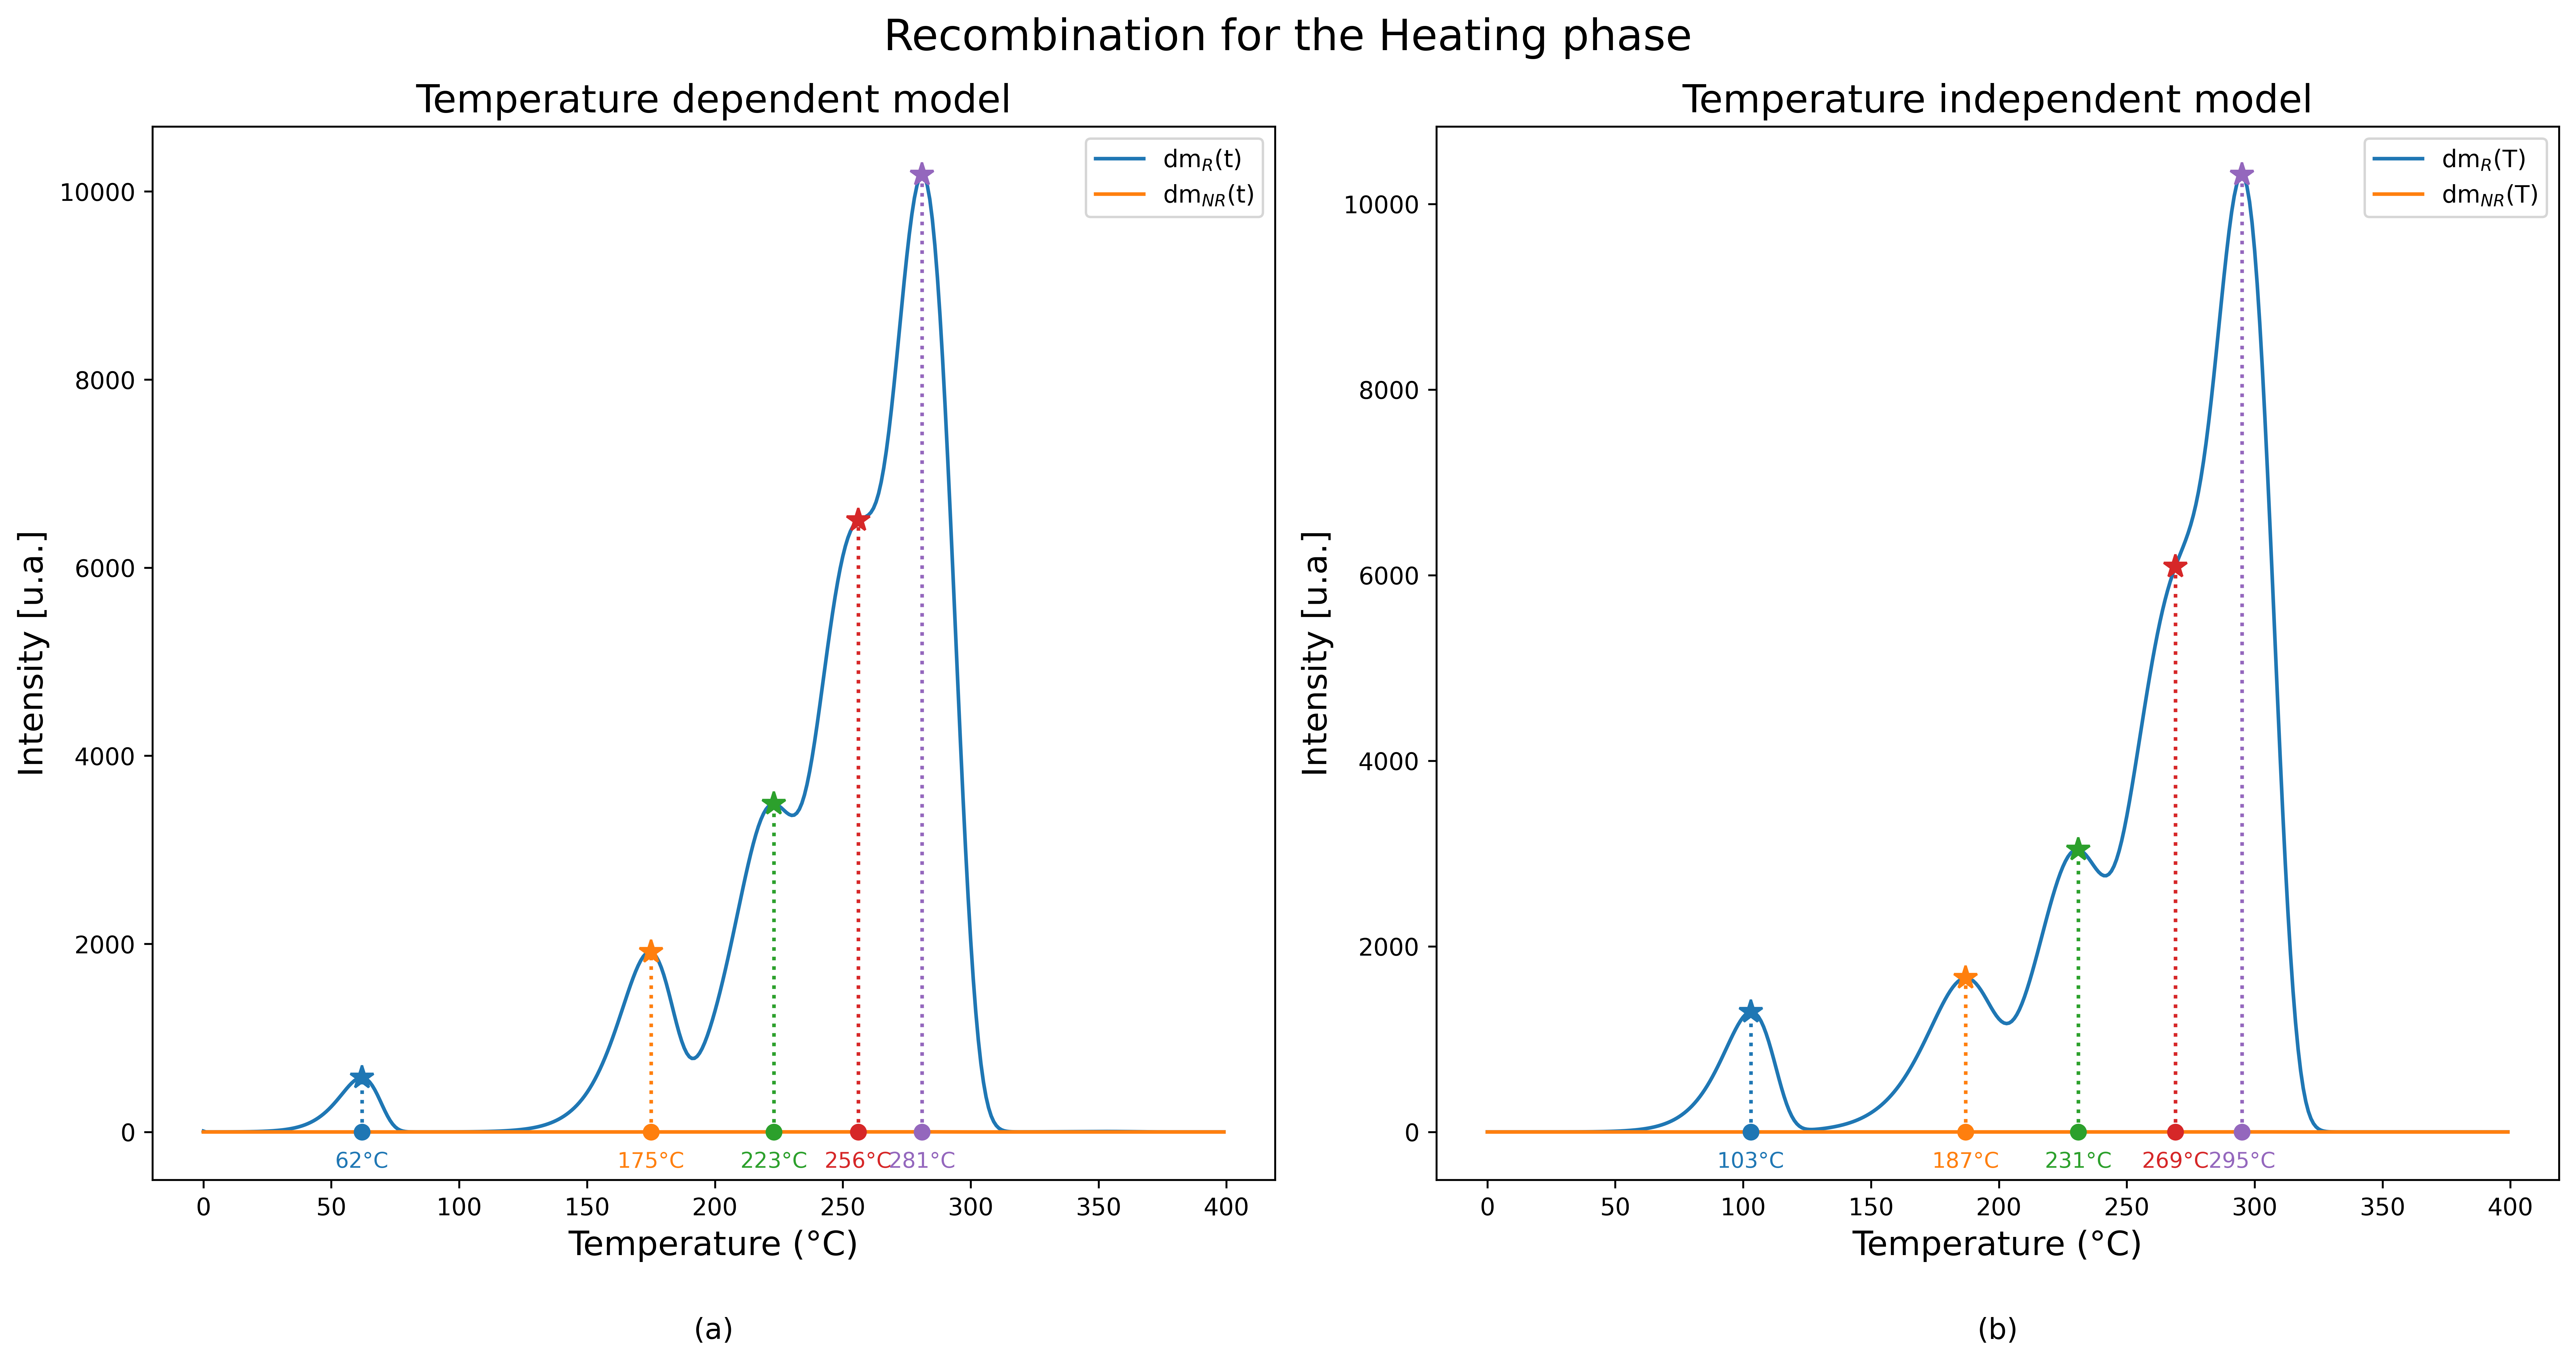
\includegraphics[width=\textwidth]{Images/GC_GlowCurve.png}
    \caption{Thermoluminescence (TL) glow curves for the LiF:Mg,Ti material plotted against temperature during the heating phase for both models. (a) Temperature dependent model; (b) Temperature independent model. The curves correspond to the radiative recombination rate $dm_R/dt$, showing the intensity of light emitted as trapped carriers recombine. For each visible peak, both the activation temperature (filled circle) and the peak temperature (star icon) are indicated. A vertical dotted line extends from each peak temperature to the X-axis, where the temperature value is labeled. The simulations were performed under a constant generation rate of $G = 0$ cm$^{-3}$ s$^{-1}$ and an increasing laboratory temperature from 0 \textdegree C to 400 \textdegree C during 400 seconds. The traps are labeled as follows: I (blue), II (orange), III (green), IV (red), V (purple), and s (brown).}
    \label{fig:heating_TLGlowCurve}
\end{figure}

And now finally, we can obtain the TL glow curve from the simulations. In Figure \ref{fig:heating_TLGlowCurve} we can see that both models display the five distinct peaks of LiF:Mg, Ti, ranging from $\sim$ 60 \textdegree C to nearly $\sim$ 300 \textdegree C, and reflects the increasing activation energies and thermal stability of the traps involved, as the peaks that appear at higher temperatures have higher luminiscent response. Comparing both models reveals that the inclusion of temperature dependency in the frequency factor slightly shifts peak positions and modifies peak intensities, particularly in shallower traps. This suggest that the temperature depencency in the frequency factor influences the occupancy dynamics of lower-energy traps. 

\vspace{10pt}

Furthermore, we can see that indeed the peak temperature values from \ref{fig:GC_ActivationAndPeakTemperatures} closely match those observed in the TL glow curve for both models. This strong agreement confirms that the temperature at which each trap empties coincides with the point of maximum luminescence intensity in the glow curve. Physically, this reinforces the interpretation that the TL glow peak directly reflects the maximum rate of carrier release from traps. The fact that this correspondence holds in both models despite their fundamental difference suggests that the thermal release of charge carriers is primarily governed by the intrinsic trap properties ---such as activation energy, trap activation temperature and frequency factor--- rather than by the specific thermal history prior to heating. This implies that the glow peak position is a robust indicator of trap characteristics, such as their activation mechanism, and luminiscent response. 

\vspace{10pt}

As a final note, we can check the validity of the model by looking at the charge neutrality condition, which can be seen in Figure \ref{fig:heating_chneutrality}. As we can see, there is a deviation from the ideal value of 1. A plausible explanation for this is that the temperature increase during the heating phase leads to a higher mobility of the charge carriers. As the temperature increases rapidly during heating, small numerical imbalances between positive and negative charges can become amplified. This is particularly true for the temperature dependent model, where the frequency factor is a function of temperature, leading to a more pronounced effect. Nonetheless, the results still offer a meaningful approximation to the expected physical behavior.

\begin{figure}
    \centering
    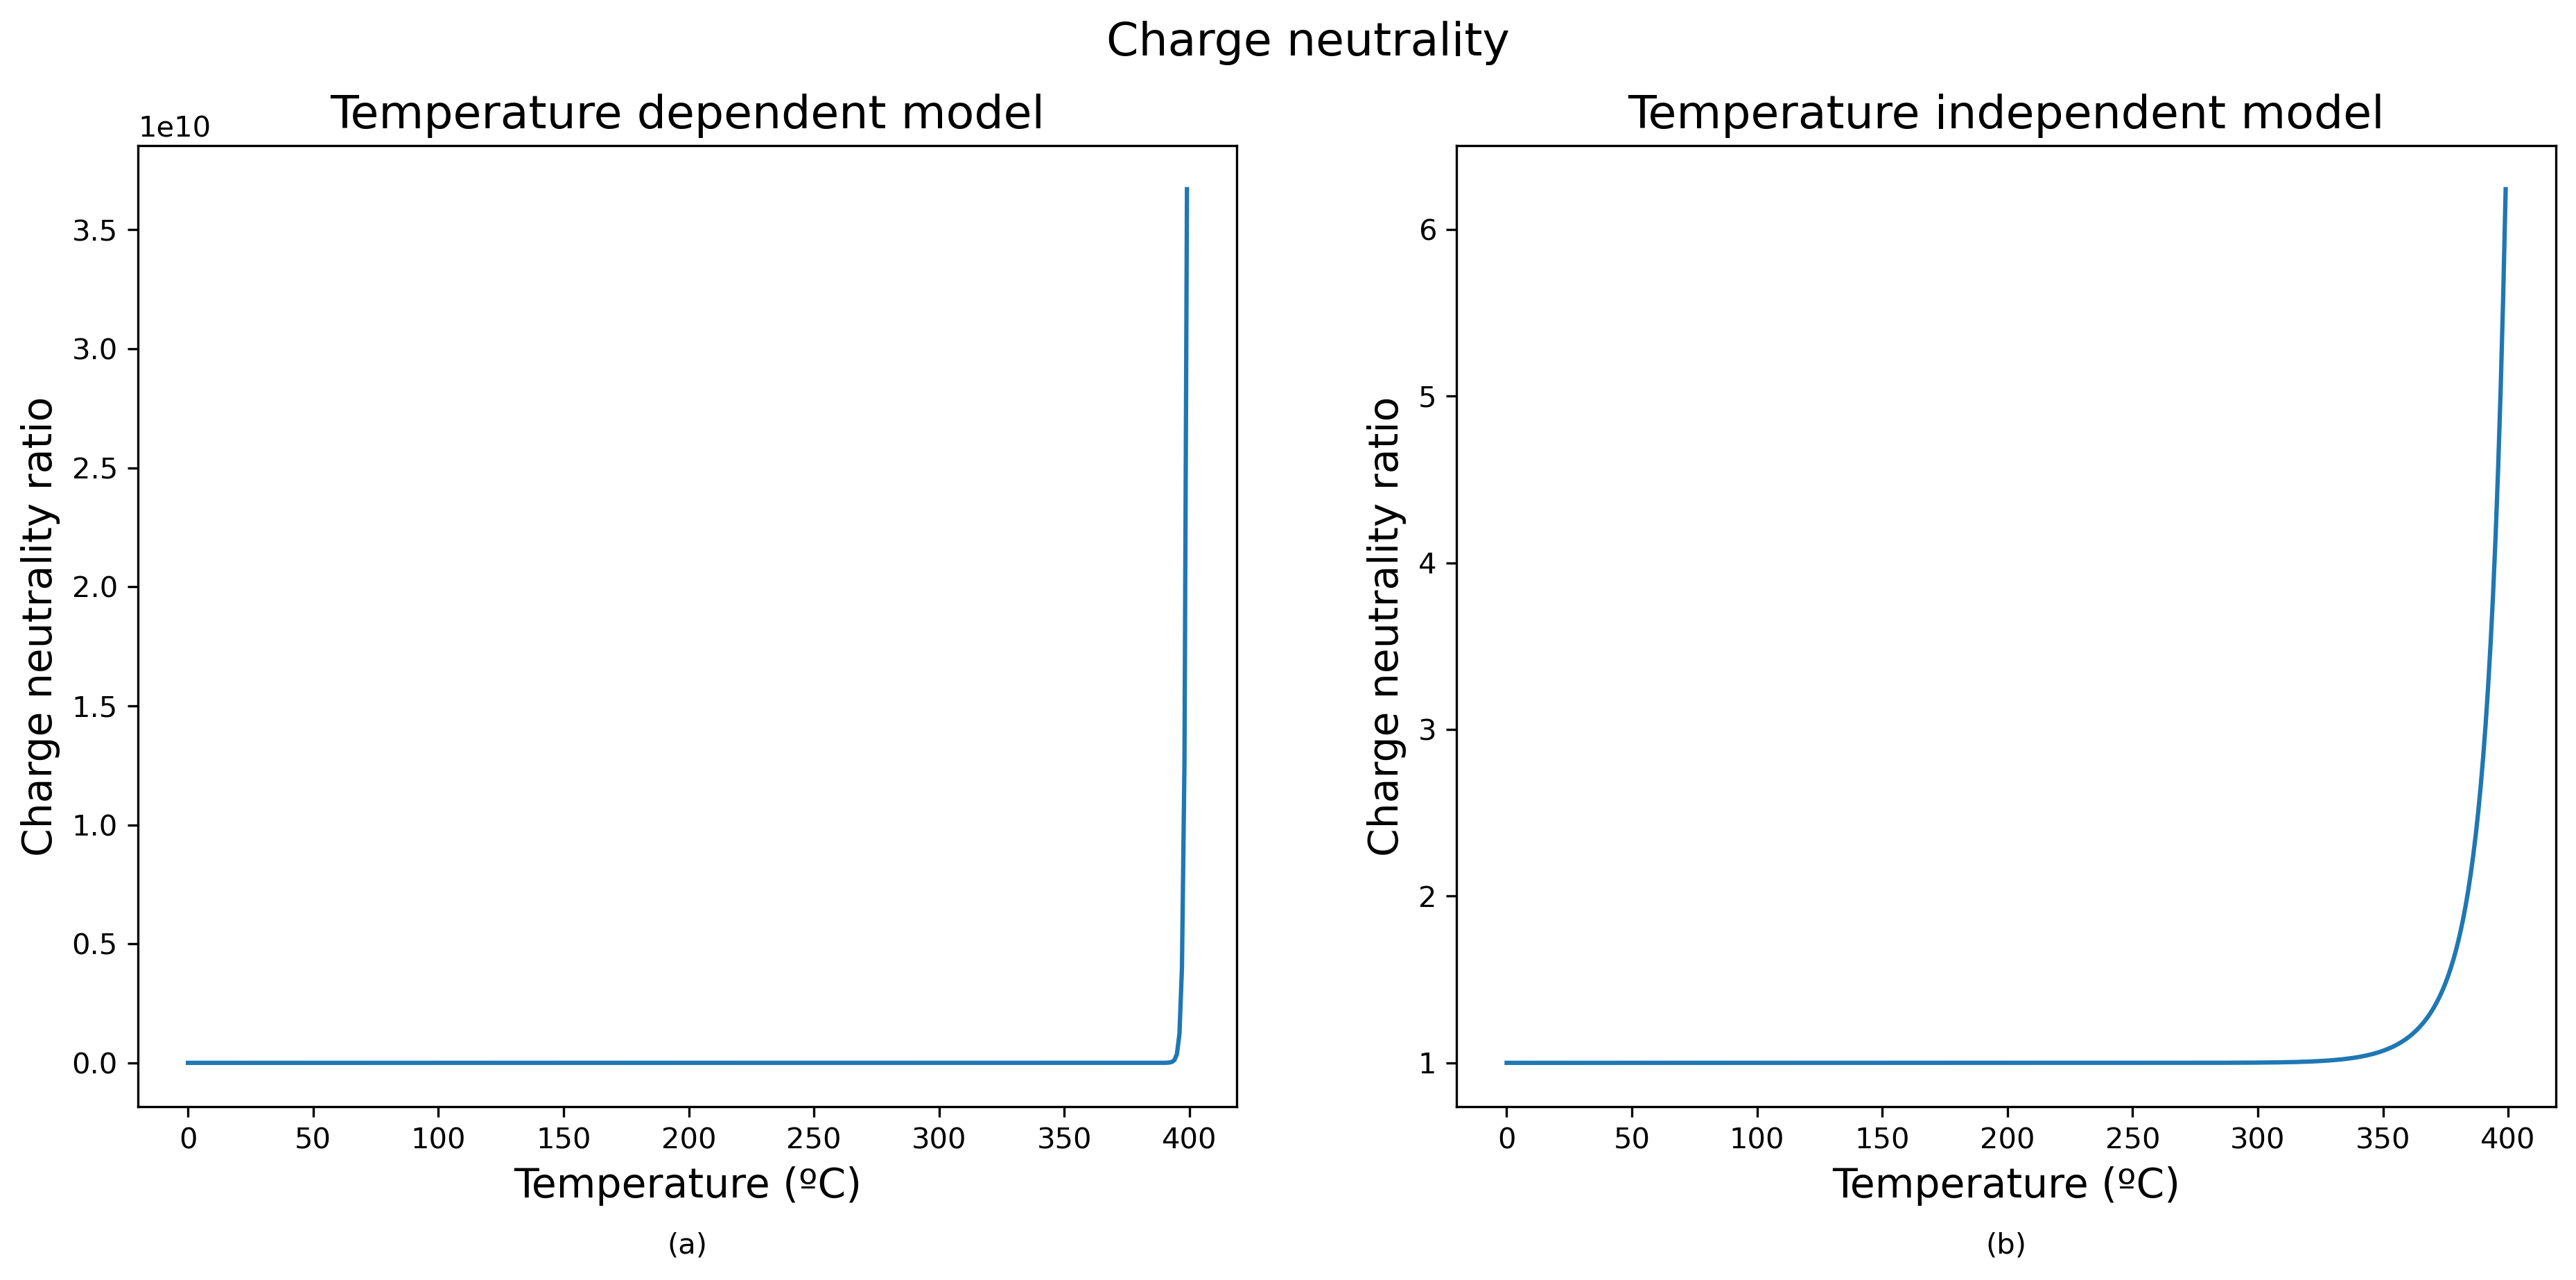
\includegraphics[width=\textwidth]{Images/Heating Charge neutrality.png}
    \caption{Charge neutrality ratio for the LiF:Mg, Ti plotted against temperature during the heating phase for both models. (a) Temperature dependent model; (b) Temperature independent model. The plotted ratio corresponds to the total negative charge divided by the total positive charges in the system. Both simulations were performed under a constant generation rate of $G = 0$ cm$^{-3}$ s$^{-1}$ and an increasing laboratory temperature from 0 \textdegree C to 400 \textdegree C during 400 seconds.}
    \label{fig:heating_chneutrality}
\end{figure}